\chapter{Analyse, Fortolkning og resultateri}
\label{Ch:4}

I dette afsnit skal vi se på det data materiale som er blevet indsamlet i forbindelse med hhv. spørgeskemaet og de skriftlige produkter. 

\section{Spørgeskemaet}
\label{Sec:4.1}

I dette afsnit belyses den empiri som er blevet indsamlet med Survey-Xact forud for elevernes skriveproces. Spørgeskemaet har indsamlet 117 besvarelser og er gennemført udelukkende i 1.g STX klasser på Viborg Katedralskole. Eleverne har skullet vurderer 5 udsagn på en skala fra 1 til 7. På denne skala var 1 meget uenig med udsagnet mens 7 var meget enig i udsagnet. 
På figur \vref{fig:4.1.a} ses det at eleverne generelt har en høj vurdering af deres udbytte af eksperimenterne som forberedelse til det forestående skrive arbejde. 

\begin{figure}[h!]
	\centering
	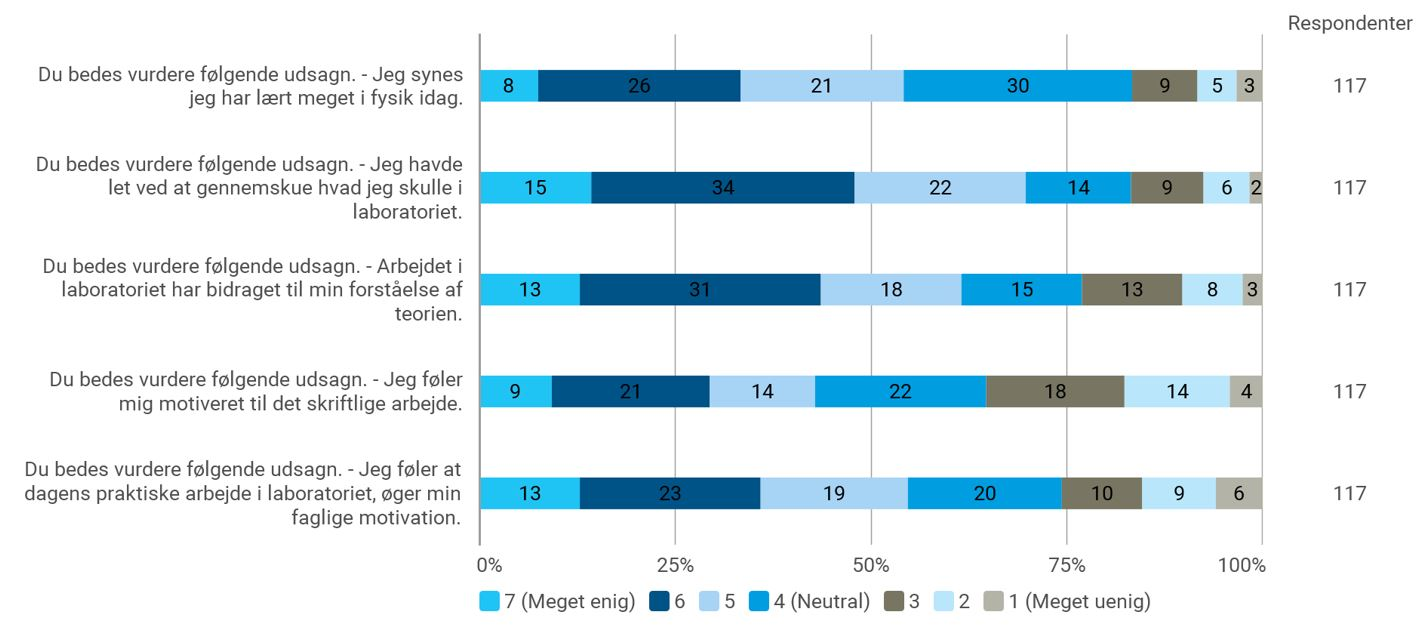
\includegraphics[width=0.9\textwidth]{Figs/Sammenlign}
	\caption{Sammenligning af de resultater som er indsamlet med spørgeskemaet.}
	\label{fig:4.1.a}
\end{figure}

Til alle fem spørgsmål i figuren udgør svarene fra neutral til meget enig i gennemsnit 66,32 \% det lader altså til baseret på dette relativt smalle datasæt at eleverne føler at de motiveres af det praktiske arbejde.

\begin{figure}[h!]
	\centering
	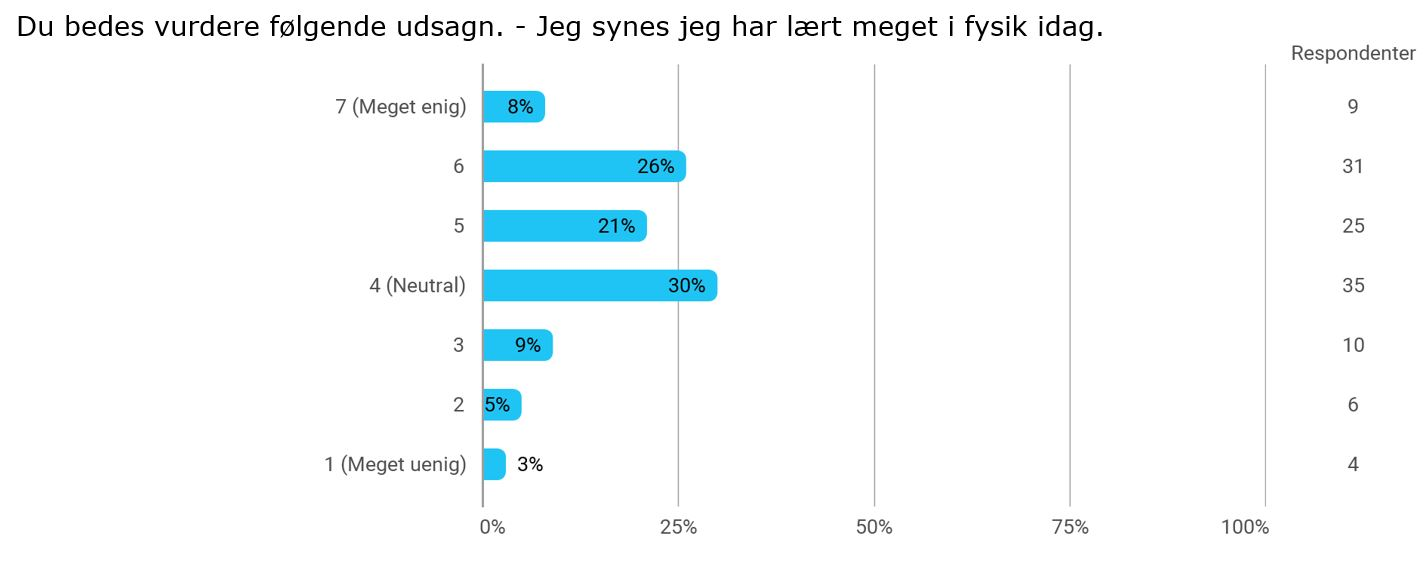
\includegraphics[width=0.9\textwidth]{Figs/Sp1}
	\caption{Spørgeskema svar fra spørgsmål 1.}
	\label{fig:4.1.b}
\end{figure}


\begin{figure}[h!]
	\centering
	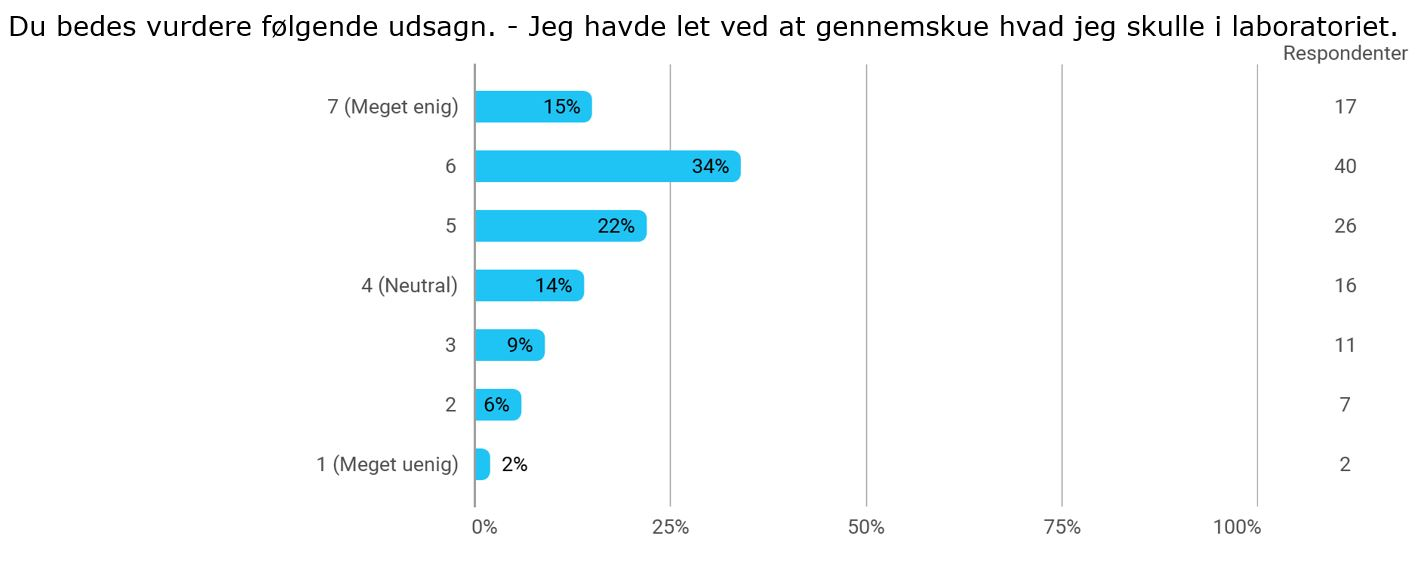
\includegraphics[width=0.9\textwidth]{Figs/Sp2}
	\caption{Spørgeskema svar fra spørgsmål 2}
	\label{fig:4.1.c}
\end{figure}

\begin{figure}[h!]
	\centering
	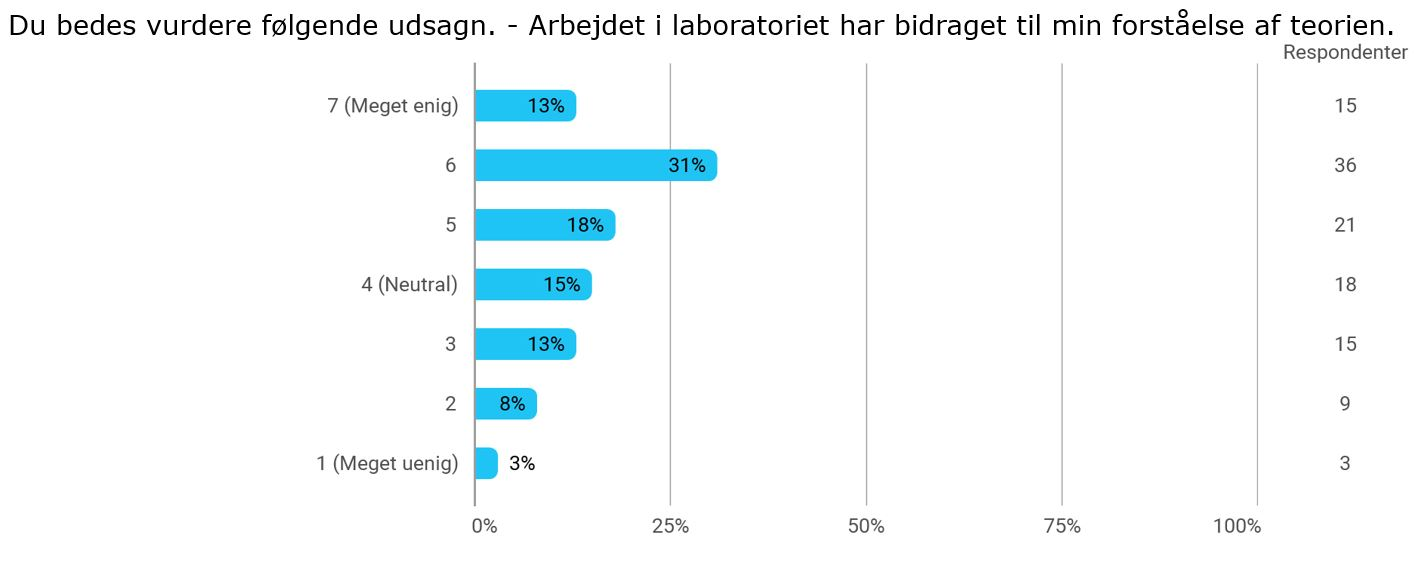
\includegraphics[width=0.9\textwidth]{Figs/Sp3}
	\caption{Spørgeskema svar fra spørgsmål 3}
	\label{fig:4.1.d}
\end{figure}

\begin{figure}[h!]
	\centering
	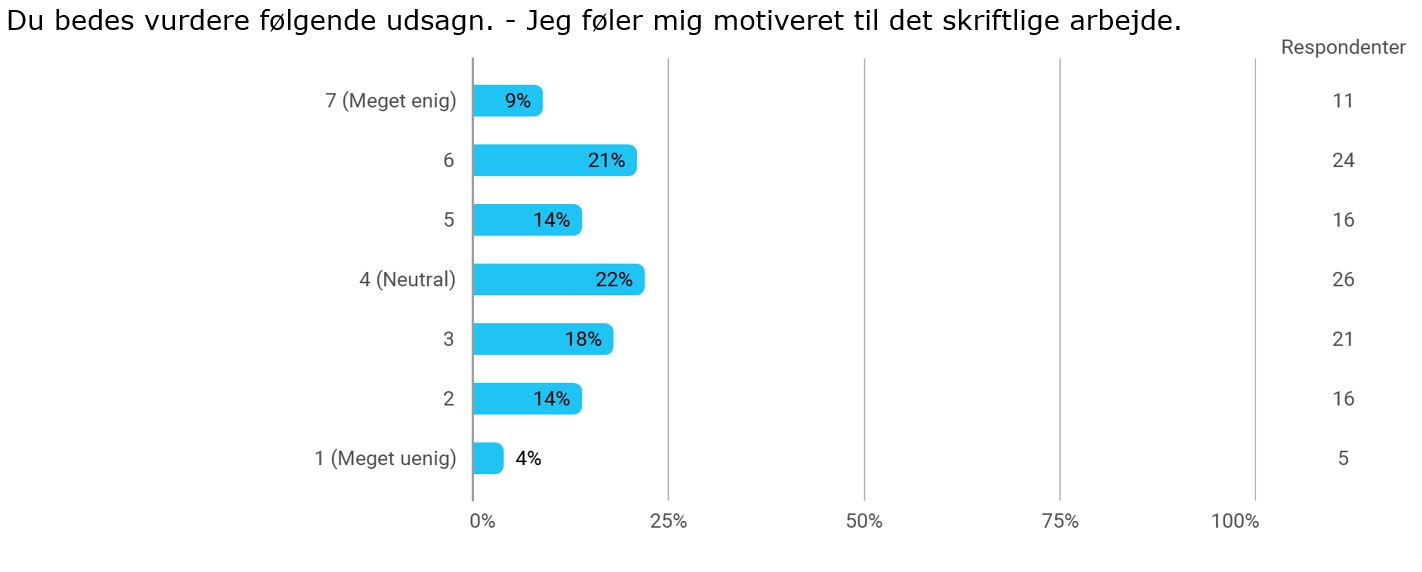
\includegraphics[width=0.9\textwidth]{Figs/Sp4}
	\caption{Spørgeskema svar fra spørgsmål 4}
	\label{fig:4.1.e}
\end{figure}

\begin{figure}[h!]
	\centering
	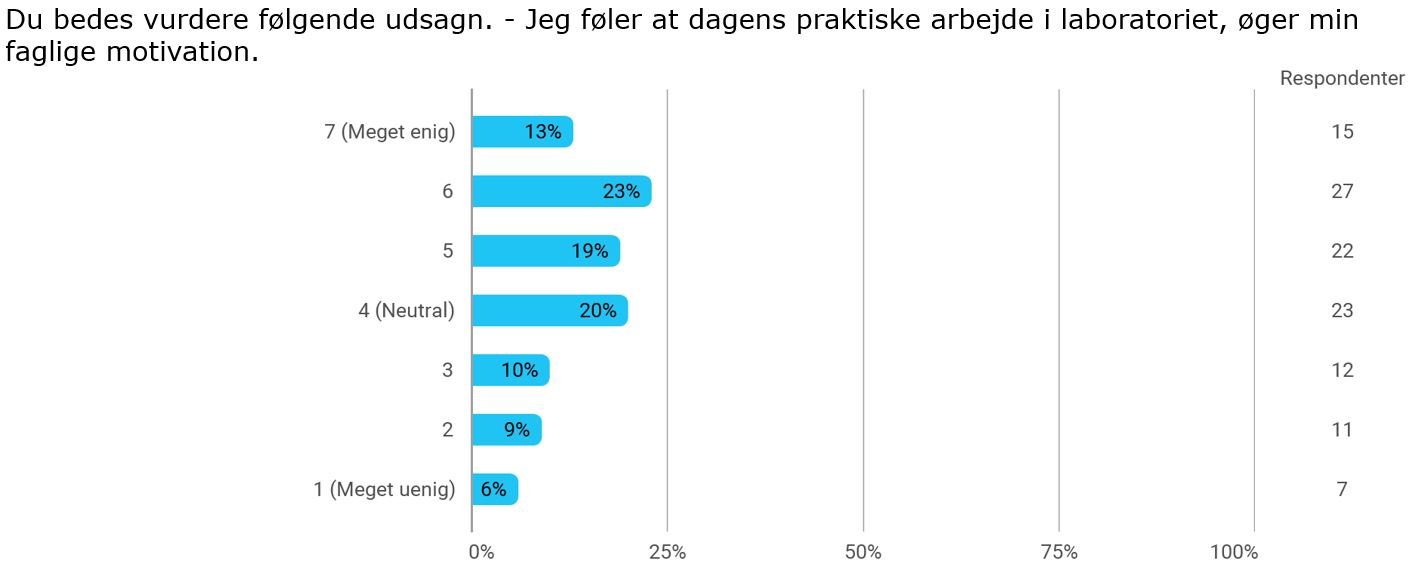
\includegraphics[width=0.9\textwidth]{Figs/Sp5}
	\caption{Spørgeskema svar fra spørgsmål 5}
	\label{fig:4.1.f}
\end{figure}
